%File: formatting-instruction.tex
\documentclass[letterpaper]{article}
\usepackage{aaai}
\usepackage{times}
\usepackage{helvet}
\usepackage{courier}
\usepackage{graphicx}
\usepackage{xcolor}
\usepackage{natbib}
\usepackage{amsmath}
\bibliographystyle{aaai}
% Sudo Code packages
\usepackage[ruled, linesnumbered]{algorithm2e}

\usepackage{amsfonts}

%\graphicspath{{C:/Users/Admin/OneDrive/Documents/School/CS-4080 Reinforcement Learning/ParkinglotANN/Images/ }}
\graphicspath{{C:/Users/Admin/OneDrive/Documents/School/CS-4080 Reinforcment Learning/ParkinglotANN/Paper/Images/}}

\frenchspacing
\setlength{\pdfpagewidth}{8.5in}
\setlength{\pdfpageheight}{11in}
\pdfinfo{
/Title (Reinforcement Learning: Parking lot)
/Author (Robert Horton)}
\setcounter{secnumdepth}{0}  
 \begin{document}

% The file aaai.sty is the style file for AAAI Press 
% proceedings, working notes, and technical reports.
%
\title{Reinforcement Learning\\ Artificial Neural Network: Valet Parking Lot }
\author{Robert Horton\\
UCCS\\
1420 Austin Bluffs Pkwy,\\
Colorado Springs, Colorado 80918\\
}
\maketitle

% ----------------------------------------------- Abstract
\begin{abstract}
\begin{quote}
With an off-policy approach the machine can be trained through different types of algorithms and parameters to influence the rate at which the policy is found and how optimal the policy found will be. By performing different training sessions with different types of learning agents of varying valued parameters and implementation, the machine can be expected to obtain better or worse optimal policies.  One popular and well know algorithm is known as the Q-Learning algorithm.  This algorithm although simple and highly effective can be written and applied in such a way that differently structured \textit{artificial neural networks} (ANN) can be implemented to use it.  Through already existing libraries this can be easily applied to any coded learning environment.  Through personal implementation and observation of these types of algorithms and varying parameters, the difference amongst these learning agents will be established and the findings there of. This study will also include the works done in other scholarly works pertaining to differently structured ANN training methods. For this implementation a simple parking lot environment will be rendered in which the machine can learn the optimal policy in which to perform parking a car.

\end{quote}
\end{abstract}

% ----------------------------------------------- Introduction
\section{Introduction}

To study and observe the differences in the various kinds structured artificial neural networks, an environment that is constricted to certain movements is an ideal test environment to observe and study how these agents behave and how optimal there  established polices might be. A simple representation of someone trying to park a car in a parking lot is a great example. Inside parking lots there are general rules that should be followed just like rules that should be followed on the road and although most parking lot can be small and simple to navigate not all are built the same and can be big and confusing to navigate. Sometimes the moves the driver can make are restricted with one way lanes and other boundaries such as medians, walkways, parked cars, and other parking spaces. Often there are big arrows and ”Do Not Enter” signs to help drivers navigate the parking lot. These different parking lots can sometimes be hard to navigate unless you are familiar with the parking lot, corresponding obstacles, and quickest parking spots. Of course overtime after navigating through the same parking lot, you learn the best way to navigate the parking lot and it becomes easier and easier to find the parking spot you want. Sometimes the easiest thing to do when looking for a parking spot it to simply pull into to first one you see but sometimes the parking spot closest to the entrance of the store that you are going to is located on the other side of the parking lot from the entrance. Such factors can sometimes affect the policy in which a desired parking spot is navigated to and parked in. Ultimately, once a parking lot has become familiar and the driver knows how to get to ”their” parking spot, they can usually use this information to navigate to other parking spots. From a machine perspective this type of information can be easily represented, stored and
shared amongst different learning agents once again making it a great testing environment for implementing off-policy learning machines. Furthermore the agents can be programmed to show verbose information and metrics, such as time, steps taken, total accumulative rewards, steps taken, calculations, and so on.  This will allow us to compare and evaluate which structured artificial neural network works the best and is more probable to find the most optimal policy when parking a car.  Other dynamic features were coded into this environment to allow the user of this program to set the size of the parking lot, amount of barriers and parking spots, location of  barriers and parking spots, and even the entrance for where the car will start at the beginning of each episode.    

% ----------------------------------------------- Background
\section{Background}

For the testing environment that our learning agents will be trained in, the parking lot size by default will be represented as a six by seven array where where each state represents an element in the array. With the agent controlling the car we can imagine each state in the parking lot represents the space that could be occupied by the car and the car can only occupy and move to one state as a time. The car is constrained to the outer bounds of the parking lot where the only entrance and exit by default is at the bottom right corner of the parking lot. There is also barriers which the car can not move move into or through.  By default there is a row of four barriers along the middle row of the parking lot including the columns two through five.  In the complex implementation we see that the barriers are along the fourth and seventh row where every column has a barrier with an opening at the end and start of the rows respectively.  The parking spaces, by default, are along the bottom and top of the barriers.  In the complex implementation only one parking spot is allowed and that is the spot in the first column of the third row.   Amongst these parking spots the user can set an assigned parking spot so the agent will know where to park.  Although pulling into unassigned parking spots is a legal move implementation of negative or lesser rewards for unassigned parking spots has been implemented.  To keep the agent out of the barrier states and to avoid breaking the rule of moving  across parking spots, a dictionary of illegal moves will be constructed. Each key will be mapped to that state's action pairs where the state is represented as a set and the illegal moves as a tuple of illegal actions in that state.  After each step the state-action pair reward will be returned to the agent to update its policy.  The action selected will also be used in the step to find what the resulting state would be when performing the selected action.  This will then be used to figure out if that action taken is illegal or takes the agent into the wrong parking space.  In this case no action is performed and the agent repeats the process of performing the next step.  However, if the action is legal then the agent checks to see if the action does take them into the correctly assigned parking spot and ultimately logs the information then ends the episode.  The number of episodes that the agent is to perform is set to 10 by default but can be changed with key word argument in the \textit{parkCar(episodes = 10)} function. Figure 1 is a picture of the default simple parking lot.  Figure 2 shows a more complex parking lot which will be used to more challenge the agents and see how well they overcome the challenge.

\begin{figure}[h]
\begin{center}
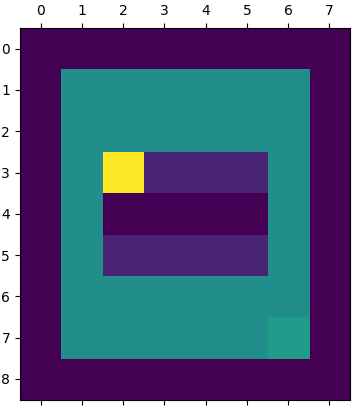
\includegraphics[scale = 0.7]{parkinglot}\\
\small{Figure 1: Default Parking lot}
\end{center}
\end{figure}

\begin{figure}
\begin{center}
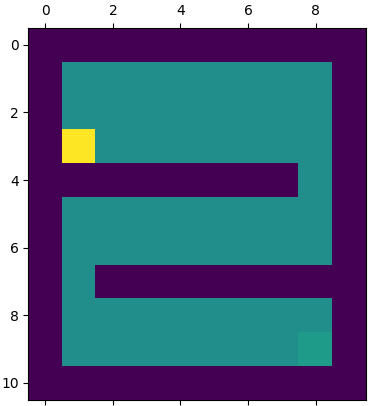
\includegraphics[scale = 0.7]{parkinglot1}\\
\small{Figure 2: Complex Parking lot}
\end{center}
\end{figure}

% ----------------------------------------------- Learning Agents
\section{Learning Agents}

Amongst the different learning agents an implementation of some kind of state-action rewards values will have to be used and so implementation of a q-learning algorithm will be used for the neural networks to use when processing different state-action rewards.  Although the various types of agents will have different versions of implemented artificial neural networks the learning agents are all required to have a limited set of actions to perform with ultimately the same goal in mind which is to park the car in the designated parking spot. A dictionary of possible parking spots can be provided with the dictionary keys set as parking spaces mapped to a directional vector that allows the agent to know which direction into that parking spot is allowed.  Each agent is allowed the same range of motion including up, down, right, and left. These actions, even though they may be illegal from a certain state, are allowed to be chosen and are used with the corresponding state values stored in the array that represents the parking lot. Illegal moves are values at -100.  Pulling into the wrong parking spots is also valued as a -100 reward.  When reaching an assigned parking spot, a reward of 100 is returned. The agents are also programmed to accept already initialized reward-table values.  Through these built reward-tables from previous training sessions the agent can use the replay memory from the reward-table to make more optimal choices on what actions to take.  
\indent Artificial neural networks is very similar to the human brain which is also one of the most intelligent things know to man today.  Through the basic concept and understanding of how the human brain works, there have been several attempts of  programming a basic artificial neural network and many of which are used today.  As a quick over view the human brain maps outs different events and observations as what can be refereed to as states or nodes.  These nodes are then linked together with otehr nodes by things called synapsis.  These synapsis then relay signals back in forth between the different nodes with different strengths.  The strength that these synapsis relay back and represent different weights with however strong the human brain might have made connection between the two nodes (\cite{Silva}).  Things like smell and sight might make the human brain make the connection between something the looks and smells good as something that will taste good and therefore want to eat it. For the purpose of this paper we want the neural network to find a better connection which set of steps will get it to it's assigned parking spot in the least amount of steps.
 
% ----------------------- Q-Learning 
\subsection{Q-Learning}

Although simplistic the concept of q-learning has been around for decades and many other forms, like the other implemented one in this paper, are based off the same concept. This simple q-learning approach gives a simplistic way of evaluating state-actions and their corresponding rewards with random actions for exploration (\cite{watkins1992q}). From the pseudocode, a simplistic and naive off policy approach of my implementation can be described.
\begin{algorithm}[h]
 \KwData{$S=\{s_1, s_2, . \ . \  ., s_{24}, s_{25}\}$,\\
 	\quad \ \ \quad $A=\{ \leftarrow, \rightarrow, \uparrow, \downarrow \}$,\\
 	\quad \ \ \quad $Q =$72 x 4 table with arbitrary values,\\
 	\quad \ \ \quad $0 \leq \gamma \leq 1$ }
 \KwResult{Find optimal policy for Parking Car}
  initialize s\;
\While{ not in parking spot}{
 \For{episode in number of episodes}{
	ExplotOrExplore = random.choice([1, 0], weight=$\gamma$) \;
	\If{1 == ExplotOrExplore}{
		$a$ = random.choice(actions) \;
	\Else{
		$a$ = S.max($Q$) \;
		}
	}
  	 perform action $a$, observe reward $r$ \& previous state $s'$ \;
	 \tiny{$Q(s,a)\leftarrow Q(s, a)+\alpha [r+\gamma Q(s',a')-Q(s,a)]\leftarrow s'$\;
	 $s \leftarrow s' $\;}
  }
}
 \caption{Q-Learning}
\end{algorithm}

However, the learning agent that use this type of implementation can be very greedy and at times if not set with the right parameters can be very stochastic (\cite{sutton2018reinforcement}).  The agent implemented with the means of how to navigate the parking lot through a list of different actions it can take.  However the way the simple q-learning agent chooses to pick which actions to take is based off of a weighted random selection between taking a exploratory action or an exploited action with the highest guaranteed reward. The weighted value for each agent is set to specific values that can vary between 0.80 - 0.99.  However with the help of any of the various different libraries available neural networks like described before can very beneficial. 


% ----------------------- Artificial Neural Network ANN 
\subsection{Artificial Neural Network (ANN) }

Like discussed before there are many different types of libraries and implementations to choose from when wanting to implement a artificial neural network into a coded learning environment.  For this implementation we used a library called \textit{keras} which is a submodule of the package \textit{tensor flow}.  With this library there are plenty of other included games to choose and deploy different learning agents to.  For this paper since we are using our own coded learning environment a simple overwritten instance of different types of neural network will be implemented and added as an abstract layer to the machine learning agents.  This abstract layer can be written to convert, retrieve, and handle the different inputs. 
\indent To implement these types of learning agents there are several things that must be considered.  First of all the activation function should be used to help mathematically describe the change in an neuron output upon different but related changes in inputs.  This is a very important component of the artificial neural network as this provide non-linearity to the output which would be usually be quite linear.  Three are several different activation functions that can be used and amongst the most popular are the sigmoid function and the rectified linear unit (ReLU) (\cite{chandrakant_2020}).\\
\begin{center}
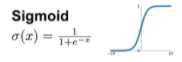
\includegraphics{sigmoid}\\
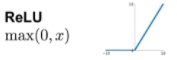
\includegraphics{ReLU}\\
\end{center}
With these functions the probability of what action will be best taken can be better represented.  Next the loss function will be found and used to find the difference between our ideal output and the actual output.  This can be called the calculated error. We use this to try and find the what is called the gradient descent.  The gradient descent is the quickest path down the slope of a modelled data set or in other words the most reward for the least amount of steps.  Essentially the artificial neural network is processing rewards for actions taken in different states and back-propagates that information to change the weights between previously taken nodes. With environments that have less memory requirements optimizers like \textit{Adam} are commonly used and will be used for this purpose of this implementation (\cite{mnih2013playing}).\\
\indent  To find all these different values and functions neural networks first randomly initializes the weights between the nodes/states and the actions that can be taken from them.  Then the machine can start to compare the output of the neural network to the ideal output to help find the error.  The machine then begins to slightly adjust the weights that seem to show a decrease in error.  This is done over and over for what ever amount of training episodes the agent has been assigned to complete.  With a learning rate hyper  parameter that controls how big the adjustment are between episodes, the user can configure the agent to make bigger or smaller connections between actions.  
\indent  To implement the artificial neural networks the inputs for the neural  networks can be implemented as the different states the agent can occupy. Within the neural network there will be individual connections between each node that is connected through a possible action. The output of the neural network represents the values for what ever action that can be taken from a given state. With these weight output values we can use these similar to q-table values and use them to take exploit actions when desired.  This can be done using the neural network by simply activating which ever input node is being occupied by the agent and getting an output of four different weight values on which action to take. To code this, different layers are simply coded to represent the input states, the dense inner layer connecting the nodes to the different state-action pairs, and lastly a layer that will help represent the output layer. For the purpose of this research paper two different types of architecture were implemented and ran on two different different test environment.\\

% ----------------------- Artificial Neural Network ANN :Type One
\subsection{Artificial Neural Network (ANN): Type One}
The architecture for the first artificial neural network was built with three layers.  Obviously the first and last layer are the input and outputs layers of the artificial neural network. The middle layer is a dense layer connecting all corresponding states to all possible moves the agent can take from that state.  This implementation also used the Adam optimizer and ReLU activation function.  As explained earlier although our layers of connected nodes and memory requirements might be big, they are relatively small for the processing power of the artificial neural network that we are using.  For that reason the rectified linear unit activation function will be used.   

% ----------------------- Artificial Neural Network ANN :Type Two
\subsection{Artificial Neural Network (ANN): Type Two}
The architecture for the second artificial neural network was built essentially the same way but instead of the input layer consisting of all nodes that are connected by corresponding  actions, we limited the connections of only nodes that are possibly connected across through legal actions only.  With this implementation we can expect the output to be even more linear and therefore use sigmoid activation function to calibrate our results. 

% ----------------------------------------------- Analysis
\section{Analysis}

Through different training sessions and observation of the results there of, several different things have been observed and concluded. Below are the results for the first artificial neural network implementation against the normal Q-Learning.  
\begin{center}
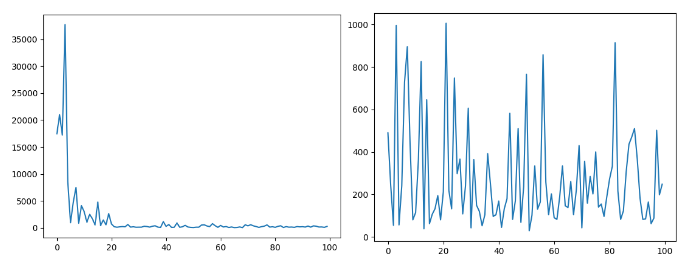
\includegraphics[scale=0.4]{ANNvsQLearning}\\
\small{Figure 3: ANN V.S. Q-Learning}
\end{center}

It is not hard to see that artificial neural network exceedingly outperforms the regular Q-learning over the range of 100 episodes.  This was also true for when the learning agents were deployed into a more complex parking lot.  Unfortunately other implementation of artificial neural networks was not able to be implemented. 
% ----------------------------------------------- Conclusion
\section{Conclusion}

In conclusion when it comes to reinforcement learning that is already so strong and simple the forefront of machine learning has been stunted by the limits in previous years of using such algorithms in such useful ways that are possible today.  Because of being constricted and limited when it comes to memory and processing power only few complex implementation of off-policy learning have been implemented that are able to look a few steps ahead at a time or minimize the error in predicted the correct actions.   However, due to recent break throughs and  development of artificial neural network libraries just about anybody can import these libraries and implement them into already existing environment or even user defined learning environments.  

% ----------------------------------------------- References 
\bibliography{ParkinglotANNArticle}

\end{document}